\documentclass[11pt,letterpaper]{report}
%%%%%%%%%%%%%%%%%%%%%%%
%% Page layout
\usepackage{graphics,graphicx,wrapfig}
\usepackage[letterpaper, margin=2.5 cm, headheight=4 cm, top= 6cm]{geometry} 
\setlength{\parindent}{0pt}
\usepackage{parskip} 
\setlength{\parskip}{0.5em}
\usepackage{todonotes}
\usepackage{fancyhdr} 
\usepackage{color}
\usepackage{soul}
\newcommand{\hlc}[2][yellow]{ {\sethlcolor{#1} \hl{#2}} }
\usepackage{comment}
\usepackage{footmisc}
% \usepackage{showlabels}
\usepackage[utf8]{inputenc}
\usepackage{tcolorbox}
\usepackage{dirtytalk}
% \usepackage{comment}

\newcommand{\eps}{0.04778cm}


    








\fancyhf{}
\fancyhead[L]{
\includegraphics[height=3 cm]{../Figures/Brown_Letterhead/H_2c_Pos}
\\
}
%
\fancyhead[C]{
\parbox[b][3.5cm][t]{4cm}{
\begin{flushright}
Haneesh Kesari
\\
Assistant Professor 
\\
of Engineering
\\
\end{flushright}
}
}
%
\fancyhead[R]{
\parbox[b][3.5cm][t]{6cm}{
\begin{flushleft}
School of Engineering
\\
Brown University
\\
184 Hope Street, B\&H 612
\\
Providence, RI 02912
\\
Phone: 401-863-1418
\\
Email: Haneesh\_Kesari@brown.edu
\\
\end{flushleft}
}
}

\fancypagestyle{plain}{
\fancyhf{} % remove everything
%
\renewcommand{\headrulewidth}{0pt} % remove lines as well
%
\renewcommand{\footrulewidth}{0pt}
%
\fancyfoot[R]{\thepage / \pageref{LastPage}}
}


%% Fonts
\usepackage{amssymb,amsfonts,amsmath,amsthm}
\usepackage{mathtools}
\usepackage[T1]{fontenc}
\usepackage{mathptmx}
\usepackage{cmbright}
\usepackage{bm}

\usepackage{sectsty}
\sectionfont{\fontsize{16}{16}\selectfont}

%% typesetting
\usepackage{tabto}

%% colors
\usepackage{xcolor}
\definecolor{DarkRed}{rgb}{0.62, 0.16, 0.09}
\definecolor{TaRed}{rgb}{0.85, 0.321, 0.153}
\definecolor{EaGold}{rgb}{0.918, 0.686, 0.122}


%% referencing
\usepackage{nameref}
\usepackage{lastpage}
\usepackage[biblabel]{cite}
\usepackage[colorlinks=true,urlcolor=DarkRed,linkcolor=DarkRed,citecolor=black]{hyperref}

%% enumerate
\usepackage{enumerate}
\usepackage{enumitem}

%% floats
\usepackage{float}
\usepackage[font=footnotesize, labelfont={bf},labelsep=period]{caption}
\usepackage{booktabs}
\usepackage{threeparttable}

%% custom commands
\newcommand{\loc}{\textit{LoC}}

\newcommand{\norm}[1]{\ensuremath \lVert #1 \rVert}

\newcommand{\ex}{{\bm{\hat{e}}}_1}
\newcommand{\ey}{{\bm{\hat{e}}}_2}
\newcommand{\ez}{{\bm{\hat{e}}}_3}
\newcommand{\ei}{{\bm{\hat{e}}}_i}
\newcommand{\ej}{{\bm{\hat{e}}}_j}
\newcommand{\er}{{\bm{\hat{e}}}_r}
\newcommand{\et}{{\bm{\hat{e}}}_\theta}
\newcommand{\ep}{{\bm{\hat{e}}}_\phi}

\usepackage{xspace}
\newcommand{\TA}{\textit{Ta.\@}\xspace}
\newcommand{\EA}{\textit{Ea.\@}\xspace}

\usepackage{etoolbox}
\usepackage{tikz}



\newrobustcmd*{\mycircle}[1]{\tikz{\filldraw[draw=#1,fill=#1] (0,0) circle [radius=0.1cm];}}

\newrobustcmd*{\mycircleTwo}[1]{\tikz{
\filldraw[draw=#1,fill=#1] (0,0) circle [radius=0.1cm];
\draw[black,thick, dash pattern={on 1.2pt off 0.5pt on 1.2pt off 0.5pt}] (0,0) circle [radius=0.1cm+\eps];
}}


\newrobustcmd*{\mytriangle}[1]{\tikz{\filldraw[draw=#1,fill=#1] (0,0) --
(0.2cm,0) -- (0.1cm,0.2cm);}}


\newrobustcmd*{\mytriangleTwo}[1]{\tikz{
\filldraw[draw=#1,fill=#1] (0,0) --(0.2cm,0) -- (0.1cm,0.173205cm);
\draw[black,thick, dash pattern={on 1.2pt off 0.5pt on 1.2pt off 0.5pt}] (-\eps*1.73205,-\eps) --(0.2cm+1.73205*\eps,-\eps) -- (0.1cm,0.173205cm+2*\eps)-- (-\eps*1.73205,-\eps);

}}



\begin{document}



%%%%%%%%%%%%%%%%%%%%%%%%%%%%%%%%%%%%%%%%%%%%%%%%%%%%%%
%%%%%%%%%%%%%%%%%%%%%%%%%%%%%%%%%%%%%%%%%%%%%%%%%%%%%%
%%%%%%%%%%%%%%%%%%%%%%%%%%%%%%%%%%%%%%%%%%%%%%%%%%%%%%
\thispagestyle{fancy}
\phantom{x}
\vspace{4em}
%Author response letter to Reviewers

\vspace{-40pt}
To: Nature Communications editors and reviewers
%hk done

Regarding: Appeal of the decision to reject the manuscript   \textit{``Architecture in Stiff Biological Materials: a Template for Toughness Enhancement, or a Siren Song?''} (NCOMMS-18-11797493)
%hk done

\vspace{3em}
Dear Editors and Reviewers,
%hk done
\vspace{1em}

Thank you so much for your consideration of our manuscript. However, we would humbly like to appeal the decision. This is because we believe that Reviewer \#1 might have misunderstood our work. In order to prevent such misunderstandings we have carried out additional experiments (see Figure~\ref{fig:NewData} of this letter) and incorporated the data from these additional experiments in the revised manuscript (see Figure 7 and Tables S1 and S2 in the revised manuscript). 
% hk done

\begin{figure}[hb!]
	\centering
	%\includegraphics[width=0.7\textwidth]{./Figures/Figure5_V7_7.pdf}
	\includegraphics[width=\textwidth]{./Figures/Figure5_V7_8.pdf}
	\caption{(a) We carried out additional experiments in which we measured fracture initiation toughness, $R(0)$, using notches that are short enough so that they lie completely outside the core region. Therefore, in these new experiments the initial crack increments can take place perpendicular to the protein interlayers. The new data from these additional experiments appear in the region $\alpha<0.19$ in the above figure (5 new data points for \textit{Ea.} and 11 new data points for \textit{Ta.}). The new $R(0)$ measurements on  \textit{Ea.}  and \textit{Ta.} spicules are marked, respectively, as \mycircleTwo{EaGold} and  \mytriangleTwo{TaRed}. The measurements reported in the original submission are shown marked as  \mycircle{EaGold} and \mytriangle{TaRed}. A modified version of this figure appears as Figure 7(A) in the revised manuscript. (b) Geometry of a fracture test specimen with a notch cut in it. A cross-sectional view shows the notch length $a$ and ligament area $A^-$.}
	\label{fig:NewData}
\end{figure}

% mm done
%hk done

We believe that our manuscript was rejected based on Reviewer \#1's comments, specifically the comment ``From their measurements, they conclude that the layered structure does not improve the fracture toughness. Unfortunately, the paper contains a serious mistake which invalidates the conclusions of the paper:''
% mm done
% hk done

We would very humbly like to suggest that Reviewer \#1 might have misunderstood the primary conclusion of our manuscript. We do not conclude, as Reviewer \#1 appears to think, that ``...the layered structure does not improve the fracture toughness.'' Our primary conclusion is that due to its cylindrical nature, the \EA spicule's layered architecture provides relatively little toughness enhancement compared to other biological materials. We state this conclusion repeatedly throughout the manuscript (both original and revised), including in the abstract where we say ``...spicule's layered architecture provides relatively little toughness enhancement,'' and in the introduction where we state ``We found that the toughness enhancement provided by the \EA spicule's architecture is much smaller than that provided by architectures seen in prototypically tough SBMs, like nacre...'' We did state that the observed increase in initiation toughness ,$R(0)$ (but not average crack growth resistance, $\left< R \right>$) was not ``significant'' (lines 177--178). We understand that our use of the word ``significant'' may have been a source of confusion. However, we chose the adjective ``significant'' in adherence with Nature Publishing Group's guidelines for reporting statistical tests. Additionally, it may also have been a poor decision on our part to report the statistical test results on our $R(0)$ measurements, since those $R(0)$ measurements corresponded to different notch lengths and it is known, e.g. from the works of Gao \textit{et al.} and Fratzl \textit{et al.}~\cite{huajian1991fracture,fratzl2007hindered, kolednik2014improvements, kolednik2011bioinspired}, that initiation toughness can change with notch length in materials with layered architectures. Therefore, it is possible that ultimately we are  responsible for Reviewer \#1's misunderstanding. We sincerely apologize for that misunderstanding and have done our utmost to reduce the chance for such a misunderstanding in the revised manuscript.
% mm done
%hk done

Our actual conclusion is less broad than the conclusion that ``the layered structure does not improve the fracture toughness.'' Despite that, our (actual) conclusion is not any less important. The interest in biological materials, such as nacre, is not due to the mere fact that their layered architecture provides toughness enhancement---this is common knowledge in the engineering community and is the underlying thesis of the entire field of composite materials---but rather due to the impressive level of toughness enhancement---by several orders of magnitude---that is seen in some biological materials (e.g., nacre and conch shell, see Figure 8 (A) and (B), in either the original or the revised manuscript). So, our finding that the \EA spicule's layered architecture provides far less remarkable toughness enhancement (in comparison to nacre by a factor of $\approx$100 in initiation toughness and by a factor $\approx$60 in average crack growth resistance) has quite an important implication. This is especially true in the biomimetics and bio-inspired engineering communities since the \EA spicule's layered architecture is being tied to potential toughness enhancement by default without determining the veracity of that enhancement through direct experiments~\cite{mayer2011new, mayer2005rigid, kolednik2011bioinspired, walter2007mechanisms}. Our work shows that  layered architecture  might not be worthy of emulation in bioinspired composites by default.   
% mm done
% hk done

Reviewer \#1 further goes to comment that ``The fracture mechanics specimens were fabricated by cutting a FIB notch into the spicules. Hereby, the notch length a varies between 0.27 and 0.4 times the diameter of the spicule (Figure 7). This means that the cut reaches the silica core of the spicule where no protein interlayers are present and the interlayers near the outside do not lie perpendicular to the crack growth direction, compare Figure 1 to Figures 3 and 6. Therefore, it is clear that the fracture resistance comes close to the fracture toughness of homogeneous calcite.''
% mm done

We completely agree with Reviewer \#1's statement above (assuming, of course, that the Reviewer meant silica when they wrote ``calcite''). In fact, from our previous work~\cite{monn2015new}, we know that roughly speaking, the notch tip would lie in the core when $\alpha>0.3$, where $\alpha$ is the dimensionless notch length $a/D$, and $a$ and $D$ are the notch length and the spicule's diameter, respectively. Thus, the Reviewer's statement that the notch reaches the core in the majority of the tests is correct. In order to have a more uniform distribution of notches, we performed additional experiments to measure initiation toughness with shorter notches (10 \EA and 14 \TA spicules).
The new measurements from these additional experiments are shown in Figure~\ref{fig:NewData} (5 new data points for \textit{Ea.} and 11 new data points for \textit{Ta.}) of this letter, and Figure 7 and Tables S1 and S2 in the revised manuscript.\footnote{We report values of $R(0)$ for only 5 out of 10 tests for the \EA spicules and 11 out of 14 tests for the \TA spicules because some of these tests exceeded limits on acceptable notch root radius size and others did not display an identifiable pop-in event. The number of tests excluded for these reasons is explained in detail in Section 2.3 and Tables S1 and S2 of the revised manuscript.}
In these additional experiments,  $\alpha<0.19$. In line with the work of Fratzl \textit{et al.}, these additional experiments show that the initiation toughness increases with decreasing $\alpha$. This is also in accordance with the statement of Reviewer \#1; in approximate parlance of Reviewer \#1, the notch tip will ``see'' more interlayers as the notch is made shorter, thereby providing the layered architecture with increased ability to enhance initiation toughness. It should be noted, however, that even for these shorter notches, the enhancement in the initiation toughness (enhancement of 4.8$\pm$3.5 (mean$\pm$standard deviation, $N$=5)) is still not as remarkable as that observed in nacre ($\approx 196$, see Figure 8 (A)). Nevertheless, the enhancement is still consistent with the work of Fratzl \textit{et al.} and Reviewer \#1's comments. We have incorporated the results from our additional experiments into the revised manuscript. In the revised manuscript we discuss these new results and our original reported measurements in the context of the works of Fratzl \textit{et al.}, and specifically state that they support the conclusions of those works (lines 209--210 in the revised manuscript).
% mm done
%hk done

Finally, we are surprised by how Reviewer \#1 could base their assessment entirely on our initiation toughness measurements and completely ignore our average crack growth resistance measurements. Different measures are used to quantify fracture toughness~\cite{anderson2017fracture, gross2017fracture, kanninen1985advanced, zhu2012review}, including critical stress intensity factors, critical energy release rate, critical $J$-integrals, and work of fracture, in addition to the ones we use, namely \textit{initiation toughness} $R(0)$ and \textit{average crack growth resistance} $\left< R\right>$. For these reasons, in the engineering fracture mechanics community, one aims to measure the $R$-curve~\cite{ritchie2011conflicts, launey2009fracture}. Albeit that different measures might be more important in different contexts (e.g., different loading scenarios) and are equivalent in certain cases (e.g., linear elastic, isotropic, homogeneous solids), the average crack growth resistance (average value of the $R$-curve) is one of the most important measures of fracture toughness when the complete $R$-curve is not available. Thus, our result that the layered architecture's ability to enhance average crack growth resistance falls from $\approx 150$ in nacre to $\approx 2.37$ in the \EA spicule (see Figure 8 (B) in the revised manuscript) due to its cylindrical nature is quite significant.    
% mm done
% hk done

Based on our above clarification of the conclusions of our work, the validity of those conclusions (e.g. their agreement with the work of Fratzl \textit{et al.}) and their importance, we hope that Reviewer \#1 would be so kind as to give our work another look.
% mm done

Also, since the concepts used in our work are related to the field of fracture mechanics and mechanics of composite materials, we request that the Editors also solicit comments from an additional fourth Reviewer with expertise in experimental or theoretical fracture mechanics or with the same expertise as Reviewer \#1.
% mm done
%hk done

We have studied the points raised by  Reviewers \#1--\#3 very carefully and have made major revisions to our manuscript in order to address those points. We have put a substantial amount of thought and effort into making our revisions. We hope that these revisions address the Reviewers' points satisfactorily. We are submitting our revised manuscript along with this letter. All the revisions  we made to our manuscript are listed in the section \textit{List of Changes} (\textit{LoC}) of this letter.
The regions containing our revisions are marked in red in the revised manuscript. 
% mm done
%hk done

We  provide a point-by-point response to the Reviewers' comments in the following pages. Our responses to Reviewer \#1's, Reviewer \#2's, and Reviewer \#3's comments can be found on pages \pageref{rev1}, \pageref{rev2}, and \pageref{rev3}, respectively, of this response letter.  In our responses we also explain how the major revisions we made address the points raised by the Reviewers. 
% mm done
%hk done

We hope that our revisions and responses are satisfactory to the Reviewers, and that they allay any concerns  you might have had about our manuscript. We thank you for your consideration of our appeal.
% mm done

\vspace{2em}
Sincerely,

Michael A. Monn, Kaushik Vijaykumar, Sayaka Kochiyama, and Haneesh Kesari


%%%%%%%%%%%%%%%%%%%%%%%%%%%%%%%%%%%%%%%%%%%%%%%%%%%%%%
%%%%%%%%%%%%%%%%%%%%%%%%%%%%%%%%%%%%%%%%%%%%%%%%%%%%%%
%%%%%%%%%%%%%%%%%%%%%%%%%%%%%%%%%%%%%%%%%%%%%%%%%%%%%%
\clearpage
\pagestyle{plain}
\newgeometry{margin=2.5 cm}
%%%%%%%%%%%%%%%%%%%%%%%%%%%%%%%%%%%%%%%%%%%%%%%%%%%%%%
\section*{List of Changes}
\label{LoCpage}

{\bf Changes in response to major Reviewer criticisms}
\begin{enumerate}[label=\textit{Mc.\arabic*}]
%

\item \label{Mc03} In response to Reviewer \#1's comments (listed as comments~\ref{r1c1b}--\ref{r1c5} of this letter) regarding the length of notches used in this work, we performed additional experiments on 10 \EA and 14 \TA spicules. From these additional experiments we report new values of $R(0)$ and $\left< R \right>$. The following changes were made as a result of these new experiments.
%
\begin{enumerate}[label=\textit{\ref{Mc03}.\roman*}]
    %
    \item \label{mc01} Modified Table 1 to reflect the 10 additional \EA specimens and 14 additional \TA specimens that we tested.
    %
    \item \label{mc02} Updated the number of \EA and \TA spicule specimens in the first paragraph of the Results section to reflect the additional \EA and \TA specimens that we tested.
    %
    \item \label{mc04} Changed the number of specimens excluded from the calculation of $R(0)$ due to excessive notch root radius or lack of pop-in in paragraph four of Section 2.3.
    %
    \item \label{mc05} Modified the fifth paragraph of Section 2.3 to update the values of $R(0)$ and to discuss the increase in fracture initiation toughness observed with decreasing notch length.
    %
    \item \label{mc06} Updated the number of specimens used to compute $\left< R \right>$ and values of $\left< R \right>$ in Section 2.4 to reflect the additional \EA and \TA specimens that we tested.
    %
    \item \label{mc07} Modified the values for the fracture toughness enhancements given in Section 2.5 and added a sentence to describe the additional enhancement in $R(0)$ observed for short notches.
    %
    \item \label{mc03} Updated the measurements of $r_n$ in the fourth paragraph of Section 2.3 to reflect the additional \EA and \TA specimens that we tested.
    %
    \item \label{mc09} Updated notch width values in Section 5.2 to reflect the additional \EA and \TA specimens that we tested.
    %
    \item \label{mc010} Updated Figure 7 and Figure 8 to include the additional \EA and \TA specimens that we tested.
    %
    \item \label{mc011} Updated Tables S1 and S2 in the Supplementary Information to include information for the additional \EA and \TA specimens that we tested.
    %
    \item \label{mc00} Added Sayaka Kochiyama as a co-author on the paper following her contributions preparing, testing, and analyzing the 10 additional \EA and 14 additional \TA specimens. 
    %
\end{enumerate}

\item \label{Mc01} In response to Reviewer \#1's comment (listed as comment~\ref{r1c1} of this letter) regarding our finding that the toughness enhancement provided by the \EA spicule's architecture is small compared to the enhancements observed in other biological materials, we have added three sentences to the abstract that clarifies the scope of these findings.
%
\item \label{Mc02} In response to Reviewer \#1's comment (listed as comment~\ref{r1c1} of this letter) regarding our finding that the toughness enhancement provided by the \EA spicule's architecture is small compared to the enhancements observed in other biological materials, we have added several sentences to the second to last paragraph of the introduction to point out that we observe a substantial increase in fracture initiation toughness for short notches and to compare this increase to previous predictions in literature.
%
\item \label{Mc04} In response to Reviewer \#1's comment (listed as comments~\ref{r1c1b} and \ref{r1c6} of this letter) regarding the length of notches used in this work, we added a paragraph following the fifth paragraph of Section 2.3 to discuss possible reasons for the increase in $R(0)$ with decreasing $\alpha$, and connect this observed increase to previous works.
%
\item \label{Mc04b} Added an acknowledgement to Reviewer \#1 for pointing us to the works of Fraztl \textit{et al.}, Kolednik \textit{et al.} and Sistaninia \textit{et al.}, which we use to explain the observed increase in initiation toughness with decreasing notch length (see comment \ref{r1c6} of this letter).
%
\item \label{Mc1} In response to Reviewer \#2's suggestion (listed as comment~\ref{r2c2} of this letter) regarding identifying the limitations of the Regularized Variational Fracture Theory, we have added a paragraph to Supplementary Information Section S4.1 that discusses the primary limitation of RVFT as it applies to the current study. 
%
\item \label{Mc2} In response to Reviewer \#2's comment (listed as comment~\ref{r2c7} of this letter) regarding inclusion of statistics both for measurements obtained in this work and those referenced from other works, we have included a new table (Table 1 in the revised version) that summarizes statistical data for specimen geometry (i.e., span, diameter, and notch length) as well as references to this table in the text.
%
\item \label{Mc3} In response to Reviewer \#2's comment (listed as comment~\ref{r2c7} of this letter) regarding inclusion of statistics both for measurements obtained in this work and those referenced from other works, we have included the standard error of the notch root radius measurements in paragraph 4 of Section 2.3 in the revised version.
%
\item \label{Mc4} In response to Reviewer \#2's comment (listed as comment~\ref{r2c7} of this letter) regarding inclusion of statistics both for measurements obtained in this work and those referenced from other works, we have modified Table 2 in the revised version to include statistical data when available for the values of $R(0)$ and $\left< R\right>$ for the other SBMs shown in Figure 8.
%
\end{enumerate}

{\bf Changes in response to minor Reviewer criticisms}
\begin{enumerate}[label=\textit{mc.\arabic*}]
%
\item \label{mc08} Added an additional point to Figure 8 to identify the approximate value of the maximum $R(0)$ enhancement observed in the \EA spicules.
%
\item  \label{mc1} Added a sentence to the first paragraph of the introduction to address Reviewer \#2's criticism that is listed as comment~\ref{r2c3} of this letter.
%
\item  \label{mc2} Modified Figure 3 and its caption, and added a figure reference to the fourth paragraph of the introduction to address Reviewer \#2's criticism that is listed as comment~\ref{r2c4} of this letter.
%
\item  \label{mc3} Modified the caption of Figure 8 and added a figure reference to the second paragraph of Section 2.5 to address Reviewer \#2's criticism that is listed as comment~\ref{r2c5} of this letter.
%
\item  \label{mc4} Modified Figure 9 to address Reviewer \#2's criticism that is listed as comment~\ref{r2c6} of this letter.
%
\item  \label{mc5} Modified the caption of Figure S1 to address Reviewer \#2's criticism that is listed as comment~\ref{r2c8} of this letter.
%
\item  \label{mc6} Modified the sentence on line 76 of the original version to address Reviewer \#2's criticism that is listed as comment~\ref{r2c9} of this letter.
%
\item  \label{mc7} Corrected typos to address Reviewer \#2's criticism that is listed as comment~\ref{r2c10} of this letter.
%
\item  \label{mc8} Added information on standard deviation and sample numbers to Table 2 in the revised version.
%
\end{enumerate}

\clearpage
%%%%%%%%%%%%%%%%%%%%%%%%%%%%%%%%%%%%%%%%%%%%%%%%%%%%%%
\section*{Response to Reviewer \#1's comments}
\label{rev1}

\begin{enumerate}[label=\textit{1.\arabic*},wide, labelwidth=!, labelindent=0pt]
\item \label{r1c1} {\bf ``From their measurements, they conclude that the layered structure does not improve the fracture toughness.''}

We would very humbly like to suggest that Reviewer \#1 might have misunderstood the primary conclusion of our manuscript. We do not conclude, as Reviewer \#1 appears to think, that ``...the layered structure does not improve the fracture toughness.'' Our primary conclusion is that due to its cylindrical nature, the \EA spicule's layered architecture provides relatively little toughness enhancement compared to other biological materials. We state this conclusion repeatedly throughout the manuscript, including in the abstract where we say ``...spicule's layered architecture provides relatively little toughness enhancement,'' and in the introduction where we state ``We found that the toughness enhancement provided by the \EA spicule's architecture is much smaller than that provided by architectures seen in prototypically tough SBMs, like nacre...''

In the original version, we did state that the observed increase in initiation toughness $R(0)$ (but not average crack growth resistance $\left< R \right>$) was not ``significant'' (lines 177--178 in the original version). However, we chose the adjective ``significant'' in adherence with Nature Publishing Group's guidelines for reporting statistical tests. It may have been a poor decision on our part to report the statistical test results on our $R(0)$ measurements, since those $R(0)$ measurements corresponded to different notch lengths and it is known, e.g. from the works of Gao \textit{et al.} and Fratzl \textit{et al.}~\cite{huajian1991fracture,fratzl2007hindered, kolednik2014improvements, kolednik2011bioinspired}, that initiation toughness can change with notch length in materials with layered architectures. Therefore, it is possible that ultimately we are  responsible for Reviewer \#1's misunderstanding. We sincerely apologize for that misunderstanding.


We do, in fact, measure an increase in both fracture initiation toughness and average crack growth resistance. For example, we found the average enhancement in initiation toughness to be 1.07 ($N$=17). In the revised manuscript, which contains additional experiments, this enhancement is even larger---1.90 ($N$=22). Similarly, for our measurements of average crack growth resistance we found that the \EA spicule's architecture provided an average enhancement of 2.39 ($N$=19).


Our conclusion was that the observed enhancements were not as remarkable as those observed in prototypically tough biological materials. For example, the enhancement of initiation toughness and average crack growth resistance for nacre are, respectively, $\approx$196 and $\approx$150 (see Figure 8 (A), either in the original or revised manuscript).

We have consequently made two changes, which are listed as \ref{Mc01} and \ref{Mc02} in the \textit{LoC} to clarify our findings.
%
Through change \ref{Mc01} we have modified the abstract to include the magnitude of the toughness enhancements that we observed in the \EA spicules.
%
Through change \ref{Mc02} we have added a paragraph in the introduction to clarify that we did measure up to a ten fold increase in fracture initiation toughness but that this increase is small compared to the increases observed, for example, in nacre.


\item \label{r1c1b} {\bf ``Unfortunately, the paper contains a serious mistake which invalidates the conclusions of the paper''}

The Reviewer points out that our original reported value for fracture initiation toughness enhancement of 1.07 was small due to the fact that most of our notches reached the spicule core where crack growth would not be perpendicular to protein interlayers. This comment is based on the assertion that a layered structure can only improve fracture toughness if an existing crack has to cross the layers. The Reviewer points us to the works of Fratzl \textit{et al.} \cite{fratzl2007hindered}, Kolednik \textit{et al.} \cite{kolednik2011bioinspired}, and Sistaninia \textit{et al.} \cite{sistaninia2018design} as support for this assertion. 

We completely agree with the Reviewer's interpretation of our data. However, we do not understand why the notches being too long in our work to reveal the larger toughness enhancements predicted by the works of Fratzl \textit{et al.} is a serious mistake. It would be a serious mistake only if the main conclusion of our work was that layered architecture does not enhance toughness. However, as we stated in our response to the previous comments, we do not conclude that the layered architecture does not enhance toughness in \EA spicules.  We only conclude that due to its cylindrical nature, the \EA spicule's layered architecture provides relatively little toughness enhancement compared to other biological materials. 


Even though it was not what we intended to say, the small enhancement in initiation toughness of 1.07 ($N$=17) reported in our original manuscript can be interpreted to mean that we are effectively saying that ``the layered structure does not improve the fracture toughness.'' In this case, our work would appear at odds with the works of Fratzl \textit{et al.}~\cite{fratzl2007hindered}, Sistaninia \textit{et al.}~\cite{sistaninia2018design}, and Kolednik \textit{et al.}~\cite{kolednik2014improvements, kolednik2011bioinspired} and the notches used in our experiments being too long to reveal the larger initiation toughness enhancements predicted by Fratzl \textit{et al.} would indeed be a ``serious mistake.'' 

To prevent such interpretations, we have carried out additional experiments. These experiments were extremely challenging and took us close to half a year to complete. As the Reviewer anticipated, these new experiments reveal the larger initiation toughness enhancements predicted by Fratzl \textit{et al}. Specifically, the additional experiments show that the enhancement in initiation toughness is 1.90 ($N$=22) on average (as opposed to 1.07 ($N$=17) in the original manuscript), and can be as large as 10. Thus, in the revised manuscript it is clear that the enhancement in initiation toughness due to the layered architecture is not negligible, is consistent with the predictions of Fratzl \textit{et al.}~\cite{fratzl2007hindered}, Sistaninia \textit{et al.}~\cite{sistaninia2018design}, and Kolednik \textit{et al.}~\cite{kolednik2014improvements, kolednik2011bioinspired}, and in fact provides strong experimental support to those works. The changes associated with these additional experiments are enumerated in \ref{Mc03} in the \textit{LoC}. We also added a new paragraph to Section 2.3 in which we connect the finding of this work to the models for toughness enhancement presented by Fratzl \textit{et al.}, Sistaninia \textit{et al.}, and Kolednik \textit{et al.}. This change is listed as \ref{Mc04} in the \textit{LoC}.
% mm and hk done


\item \label{r1c2} {\bf ``A layered structure improves fracture toughness and damage tolerance only, if an existing crack has to cross the layers, i.e. when it propagates perpendicular to the spatial variation of the material properties, see e.g. Fratzl et al. Advanced Materials 2007 and ref. [8].''}

Assuming that the Reviewer means flat layers, we agree with the Reviewer's comment with regard to average crack growth resistance. In relation to initiation toughness, we also agree with the Reviewer's comment if the qualifier ``only'' is removed. That is, we are unable to agree that enhancement of initiation toughness is \emph{only} possible if crack growth from a notch is perpendicular to the layers.

\item \label{r1c3} {\bf ``Hereby, the notch length a varies between 0.27 and 0.4 times the diameter of the spicule (Fig. 7). This means that the cut reaches the silica core of the spicule where no protein interlayers are present and the interlayers near the outside do not lie perpendicular to the crack growth direction, compare Fig. 1 to Figs. 3 and 6.''}

We agree with the spirit of the Reviewer's comment.

However, we would like to point out that the notch lengths in our original experiments varied between 0.18 and 0.64 times the diameter of the spicule (Figure 7 and Table S1 in the original submission). In the revised manuscript, which includes data from additional experiments, the notch lengths vary between 0.07 and 0.64 times the diameter of the spicule (Figure 7 and Table S2 in the revised manuscript). From our previous work~\cite{monn2015new} we know that, roughly speaking, the notch tip would lie in the core when $\alpha>0.3$, where $\alpha$ is the dimensionless notch length, $a/D$, and $a$ and $D$ are the notch length and the spicule's diameter, respectively.  

Thus, in the original manuscript the notch tip does not reach the core in 29\% of the initiation toughness experiments (see Table S1 in the original submission), and in the revised manuscript the notch tip does not reach the core in 45\% of the initiation toughness experiments (see Table S1 in revised manuscript).

\item \label{r1c5} {\bf ``Therefore, it is clear that the fracture resistance comes close to the fracture toughness of homogeneous calcite.''}

We agree with the Reviewer's comment (assuming, of course, that the Reviewer meant silica when they wrote ``calcite'').

\item \label{r1c6} {\bf ``The increase of fracture toughness due to soft and/or compliant interlayers has been demonstrated experimentally in several papers, e.g. in Sistaninia et al., Composite Structures 2018.''}


We thank the Reviewer for pointing us to the work of Sistaninia \textit{et al.} Our work is not at odds with the results presented by Sistaninia \textit{et al.}~\cite{sistaninia2018design} or the related works of Fratzl \textit{et al.}~\cite{fratzl2007hindered} and Kolednik \textit{et al.}~\cite{kolednik2014improvements,kolednik2011bioinspired}. In fact, we now use these works to explain  the increase in initiation toughness with decreasing notch length that was revealed by our additional experiments  in the revised  manuscript.  Furthermore, we thank Reviewer \#1 in the acknowledgements section of the revised manuscript for pointing us to the works of Sistaninia \textit{et al.},  Fratzl \textit{et al.}, and Kolednik \textit{et al} and also for giving the explanation of why the initiation toughness for large notches is close to that of silica, which we have also included in the revised manuscript. See change \ref{Mc04} and \ref{Mc04b} in the \textit{LoC}.

\item \label{r1c7} {\bf ``p.4, l.54: `Roughly speaking, fracture toughness---also known as crack growth resistance, R---is the amount of energy that a crack consumes to grow its area by a unit amount.' This is valid for brittle, homogeneous materials only, but not for inhomogeneous materials where a crack has to cross soft interlayers.''}

We respectively disagree with the Reviewer. See, for example, the works by Gao~\cite{huajian1991fracture} and Hsueh \textit{et al.}~\cite{hsueh2018stress}. Consequently, we have not changed our statement that the Reviewer refers to in the revised manuscript.

\item \label{r1c8} {\bf ``p.9 Fig 5 and p.11: It is wrong to compute the fracture initiation toughness of the E. aspergillum spicule from Eq. (2). The change in potential energy and the crack extension during the the pop-in only gives the crack growth resistance for the first crack growth increment after fracture initiation.''}

We agree with second part of the Reviewer's comment, which is namely ''The change in potential energy and the crack extension during the the pop-in only gives the crack growth resistance for the first crack growth increment after fracture initiation.'' We further note that the crack growth resistance for the first crack growth increment is, by definition, the fracture initiation toughness.

However, we respectfully disagree with the first part of the Reviewer's comment, namely ''It is wrong to compute the fracture initiation toughness of the E. aspergillum spicule from Eq. (2).''

The Reviewer might be conflating the different measures of fracture toughness, specifically initiation toughness with average crack growth resistance.
Only the changes during the ``first crack growth increment after fracture initiation'' (by which we assume that the Reviewer means the limit of vanishingly small crack increments starting from when there is no crack, only notch)  are needed for computing initiation toughness, but are insufficient for computing average crack growth resistance. Thus,
Equation (2) is completely valid to compute initiation toughness.    

To clarify, we derive Eqn. (2) directly from Griffith's theory of fracture, in which a necessary condition for a crack to start growing is that the energy release rate should equal or exceed the material's crack growth resistance. That is, 
%
\begin{equation}
-\frac{d \Pi (\Delta a;\; w_s)}{d\Delta A(\Delta a;\; a,\;D)}=R(\Delta a)
\label{eq:GriffithCrack}
\end{equation}
%
where the function $\Pi(\cdot;\;w_s)$ is a function, which when supplied by the crack length $\Delta a$ returns the system's potential energy $\Pi(\Delta a;\;w_s)$.  The applied displacement  $w_s$ is a parameter in this function. On inputting the crack length  $\Delta a$, the function  $\Delta A(\cdot;\; a,\;D)$ returns the area of the fracture surface. This function is parameterized by the notch length $a$ and the spicule diameter $D$. Equation~\eqref{eq:GriffithCrack} can be found in any basic textbook on fracture mechanics, such as~\cite{gross2017fracture, anderson2017fracture, kanninen1985advanced, lawn1993fracture}.


The initiation toughness $R(0)$ is the value of the crack growth resistance $R(\cdot)$ in the limit of vanishing crack length. That is, 
\begin{equation}
R(0)=\lim_{\Delta a\to 0+}R(\Delta a).
\label{eq:InitiationToughness}
\end{equation}
Equation (2) in the manuscript follows from 
~\eqref{eq:GriffithCrack} and~\eqref{eq:InitiationToughness}.

% mm and hk done

\end{enumerate}

\clearpage
%%%%%%%%%%%%%%%%%%%%%%%%%%%%%%%%%%%%%%%%%%%%%%%%%%%%%%

\section*{Response to Reviewer \#2's comments}
\label{rev2}

\begin{enumerate}[label=\textit{2.\arabic*},wide, labelwidth=!, labelindent=0pt]

\item \label{r2c1} {\bf ``On the use of the variational fracture method (VFM) to discuss and explain the results. The set of past works from Ambrosio and Tortorelli, and later Francfort and Marigo (1998 \& 2000) report numerical evidence for the variational fracture theory validation. While I certainly acknowledge the power and refinement of this method, I wonder whether after 18-20 years, the authors could have considered adding experimental validation. This would be certainly pertinent here considering the VFM is now applied to a biological layered material.''}

We agree with the Reviewer that experimental validation is extremely important for verifying the predictive capabilities of any computational tool. While we did not include this information in the manuscript, we have carried out extensive simulations to experimentally validate our finite element implementation of the Regularized Variational Fracture Theory (RVFT). We plan on presenting those validation results in a different manuscript that is currently under preparation\footnote{``A variational mechanics theory for modeling the evolution of crack networks in composite materials with brittle interfaces,'' Kaushik Vijaykumar, Pooya Yousefi, Christopher Larsen, and Haneesh Kesari. Under preparation for submission to the \textit{Journal of the Mechanics and Physics of Solids}\label{RVFTpaper}}.  We briefly discuss three of our  RVFT experimental validation results in the following paragraphs. %hk done      



\begin{figure}[hb!]
	\centering
	\includegraphics[width=\textwidth]{./Figures/CrackPathSim_V1_ver1.pdf}
	\caption{(a)--(b) Results from the bending test performed by Clegg \textit{et al.}\cite{clegg1990simple} on a SiC-graphite layered beam. %hkdone
	(a) shows the failed configuration of the beam at the end of the bending test. %hkdone
	(b) shows the  load-displacement curve from the bending test. %hkdone
	(c)--(d) Results from  RVFT simulation of Clegg \text{et al.}'s bending test. %hkdone
	The beam in the simulation was two dimensional, i.e., we assumed plane strain conditions. %hkdone
	The SiC layers and the graphite interlayers (weak interfaces) are marked with symbols $G_{b}$ and $G_{I}$, respectively, in (c). %hkdone
	The span and width of the beam and the thicknesses of the SiC layers and interlayers are also shown marked in (c). %hkdone
	(c) shows a representative crack pattern predicted by the RVFT simulations. The cracked region (where the damage field $d$ is close to unity) is shown in red. The triangular notch is 0.1 mm at the base and 0.0625 mm in height. %hkdone
	(d) shows the load-displacement curves from the RVFT simulations for different number of interlayers (weak interfaces). %hkdone
	In the simulations  toughnesses of the SiC layer and graphite interlayers were $500 \;\rm J/m^2$ and $50 \;\rm J/m^2$, respectively, and the Young's modulus and Poisson's ratio of the SiC were $20.8\;\rm GPa$ and $0.3$, respectively. %hkdone
	}
	%The material properties corresponding the load-displacement data in subfigure (d) E = 20.8 *10^3 N/mm^2, $\nu$ = 0.3, l = 0.025 mm, m = 2, g_b = 0.5 N/mm, g_I = 0.05 N/mm
	%The material properties corresponding the contour plot in subfigure (c) E_b = 20.8 *10^3 N/mm^2,E_I = 2.08 *10^3 N/mm^2, $\nu$ = 0.3, l = 0.025 mm, m = 2, g_b = 0.5 N/mm, g_I = 0.1 N/mm
	%WoF SiC - 62 Jm^{-2} (upper bound), SiC-Graphite - 4625 Jm^{-2}. KIc SiC - 3.6 MPa-m^{-1/2}, GIc SiC - 28.25 Jm^{-2}, KIc SiC-Graphite 15 MPa-m^{-1/2}, GIc SiC-Graphite - 490. 478 Jm^{-2}
	% Enhancement from simulations WoF-3 interlayer/WoF-0 interlayer = 1.85, Percentage increase is (WoF-3 interlayer-WoF-0 interlayer)/WoF-0 interlayer = 85.81 %
	\label{Fig1}
\end{figure}
%hk done


\paragraph{Three point bending of a layered beam:}
Clegg et al. \cite{clegg1990simple} created a layered beam by coating Silicon Carbide (SiC) sheets with graphite and then pressing and  sintering them together. The graphite coating  creates weak interfaces between the SiC sheets. This layered beam structure can be thought of  as a 2D synthetic analogue for the \textit{Ea.} spicules, where the 
SiC sheets and graphite coating represent the \textit{Ea.} spicules' silica layers and  protein interlayers, respectively. In fact, this structure is very similar to the ``simple synthetic analogue''/``artificial layered beam'' that Reviewer \#2 mentions in their comment \ref{r2c12}. Clegg \textit{et al.} notched the SiC-graphite beam and loaded it until failure in a three-point bending configuration. (Note that we too notched the spicules and performed bending tests on them.) A failed configuration of the SiC-graphite layered beam from the bending test is shown in Figure~\ref{Fig1} (a). The load-displacement curve from the bending test is shown in Figure~\ref{Fig1} (b). 
% hk done

We simulated Clegg \textit{et al.}'s bending test using the  RVFT. The results from our RVFT simulation of Clegg \textit{et al.}'s bending test are shown in Figure~\ref{Fig1}(c)--(d). The values for some of the parameters in the simulations were different from those in the experiments. For example, the values for the toughness and stiffness of SiC  in our simulations ($500~\rm J/m^2$ and $20.8~\rm GPa$, respectively) were different from those reported by Clegg \text{et al.} for the SiC in their experiments ($28.25~\rm J/m^2$ and $450~\rm GPa$, respectively).  We chose different values because the values for some of the parameters  in Clegg \textit{et al.}'s experiments were unavailable to us, such as the total number of SiC layers, thickness of a SiC layer (although this can be estimated from the images), the length and width/thickness of the SiC-graphite layered beam, toughness of the graphite interfaces, etc. Therefore instead of attempting to match our simulation results quantitatively with the experiments, we only attempted to match them qualitatively. So, we chose the parameter values in the simulations to make the RVFT's predictions qualitatively match experimental observations  while ensuring that the RVFT computations did not become prohibitively expensive.
% hk done
 
 %%% hello
The RVFT is able to qualitatively capture  many of the salient features of the experiment. For instance,  as in the experiments  in our RVFT simulations the crack begins to grow from the notch only  when the energy release rate matches the toughness (critical energy release rate) of SiC. Also in agreement with the experiments, in our RVFT simulations the load drops after the first crack growth, the  crack gets deflected on reaching the weak interfaces (interlayers), and following each deflection there is an increase in the load. Overall, the RVFT simulated crack has the same branched appearance as the experimentally observed crack (cf. Figure~\ref{Fig1} (a) and (c)), and the  RVFT simulated load displacement curve has the same stair-step appearance as the experimentally measured load-displacement curve (cf. Figure~\ref{Fig1} (b) and (d)). Finally, the RVFT simulations are also able to capture the experimentally observed enhancement in the work of fracture provided by the layered architecture.  Clegg \textit{et al.} reported that the work of fracture for the  SiC-graphite layered beam was $4625$ J/m$^2$, while that of monolithic SiC beam was $62$ J/m$^2$. That is, in the experiments the layered architecture enhances the work of fracture $\approx 75$ times. In the RVFT simulations (containing three interlayers/weak-interfaces) the  layered architecture enhances the work of fracture $\approx 2$ times. 
% hk done
  






\paragraph{Asymmetric three point bending of a plate containing three holes}


%%
	Ingraffea and Grigoriu performed a asymmetric three-point bending test on a notched poly(methyl methacrylate) (PMMA) plate containing three holes~\cite{ingraffea1990probabilistic} (see Figure~\ref{fig:ThreeHoles} (a)--(b)). %hk done
	Here ``asymmetric'' refers to the fact that the notch was off center in the span direction (see Figure~\ref{fig:ThreeHoles} (a)). %hk done 
	The specimen's geometry and the experiment's loading are shown in Figure~\ref{fig:ThreeHoles} (a). %hk done
	Figure.~\ref{fig:ThreeHoles} (b) shows the experimentally observed crack path. %hk done
	As can be noted, the crack emanates from the notch tip, curves to the right, and terminates in the middle hole.   
	%hk done

%%%%  
	We simulated Ingraffea and Grigoriu's  experiment using the  RVFT. %hk done
	In the simulations all dimensions in the span and the width directions  were the same as those  in the experiments. %hk done
	The span and the width directions are, respectively, the $\boldsymbol{e}_1$ and $\boldsymbol{e}_2$ directions that are shown marked in Figure~\ref{fig:ThreeHoles} (a). %hk done
	In the simulations we took the specimen to have infinite thickness, i.e., the RVFT simulations were two dimensional. %hk done
	Further details of our RVFT simulations are given in Figure~\ref{fig:ThreeHoles}'s caption. %hk done

On comparing Figure~\ref{fig:ThreeHoles} (b) and (c), visually, the crack path predicted by our RVFT simulation appears to match the experimentally observed crack path quite well. %hk done
In order to quantify this match, for both the experiment and the simulation,  we select a finite number of points on the crack path and measure the angles that the tangents to the crack path at those points make with  the span direction ($\boldsymbol{e}_1$ direction in Figure~\ref{fig:ThreeHoles} (a)). %hk done
We show those angles as a function of the points' abscissa in Figure~\ref{fig:ThreeHoles} (d). %hk done
As can be seen, the crack path predicted by the RVFT indeed matches the experimentally observed crack path remarkably well. %hk done
%hk done

 


\paragraph{Shear loading of a PMMA plate containing a vertical slit at its center} %  hkdone
Erdogan and Sih have reported fracture experiments  on a  PMMA plate that contained a vertical slit at its center~\cite{erdogan1963crack}. %hkdone
The loading on the PMMA plate in the experiments is shown in Figure~\ref{fig:ErgodanSih} (a). %hkdone
The crack path observed in the experiments is shown in Figure~\ref{fig:ErgodanSih} (b). %hkdone

We modeled Erdogan and Sih's experiment using the RVFT. %hkdone
We could not ascertain the dimensions of the  PMMA plate in the experiments. %hkdone
Therefore, we chose to model only a small region around the central slit's top tip (region shown marked using dashed lines in Figure~\ref{fig:ErgodanSih} (a).i) in our simulations. %hkdone
The modeled region was   $2~\rm mm$ in both the span and the width directions and contained a notch of 1 mm length on its bottom edge (see Figure~\ref{fig:ErgodanSih} (b)). %hkdone
The notch was parallel to the width direction. %hkdone
The span and the width directions are, respectively, the $\boldsymbol{e}_1$ and $\boldsymbol{e}_2$ directions that are shown marked in Figure~\ref{fig:ErgodanSih} (b). %hkdone
The loading on the modeled region in the simulations is also shown in  Figure~\ref{fig:ErgodanSih} (b). %hkdone
All other details in the simulations were the same as those in our simulation of Ingraffea and Grigoriu's  experiment. %hkdone
%hkdone



A representative result from our RVFT simulation is shown in Figure~\ref{fig:ErgodanSih} (b). %hkdone
We measured the crack initiation angle in both the experiments and in our simulations. %hkdone
The crack initiation angle is the angle that a tangent to the crack at the point of its origin (which in the current context is the slit's top tip) makes with the width direction. %hkdone
The crack initiation angle in the experiments for  the crack shown in Figure~\ref{fig:ErgodanSih} (a).ii is $70 \pm 3^{\circ}$, while 
we found the crack initiation angle in our simulations to be $\approx 69.2^{\circ}$. %hkdone




The regularized, variational fracture theory's  predictions have been compared with experimental observations by other researchers as well, for example, see \cite{mesgarnejad2015validation},~\cite{miehe2010phase}, and ~\cite{wu2017phase}. %hk done


The three experimental validation results that we just discussed in response to Reviewer \#2's comment~\ref{r2c1}, and similar experimental validation results reported in literature make us feel confident that the  RVFT is a dependable tool for gaining qualitative insight into fracture mechanics related phenomena. %hk done
Needless to add, and as we will discuss in our response to Reviewer \#2's comment~\ref{r2c2}, the RVFT does have several limitations with regard to its predictive capability, and requires further development before it is capable of making quantitative predictions. %hk done
However, we have done our utmost to ensure that the issues that are known to limit RVFT's predictive capability were absent or negligible in the  simulations that we report in the manuscript. %hk done  

\begin{comment}
\begin{tcolorbox}[colback=red!5,colframe=red!75!black,title=To Do Sayaka]
\begin{enumerate}
    \item Is there a better term to talk about \say{glue}. Right now we are using the term \say{polymeric-adhesives}.
		\item In Figure~\ref{fig:ThreeHoles} (a) and Figure~\ref{fig:ErgodanSih} (a), include two arrows. Marks those arrows as $\hat{\boldsymbol{e}}_1=\text{Span direction}$ and $\hat{\boldsymbol{e}}_2=\text{thickness direction}$.
    \item Notch is not clear in Figure~\ref{fig:ErgodanSih} (b). There are two white lines. Perhaps changing the color of the notch to a different color would help.
    \item Need to add subfigure \textit{c} to Figure~\ref{fig:SyntheticAnalogues}, so that following text makes sense \say{Figure~\ref{fig:SyntheticAnalogues} (c) shows the mechanical testing that we have designed and constructed for carrying our three-point bending fracture tests our spicule synthetic analogues. }
		\item In Figure~\ref{fig:SyntheticAnalogues} change \say{Compliant interlaye (glue)} to "Polymeric-adhesive interlayers (PMMA-PMMA interfaces)"
\end{enumerate}


\tcblower

\end{tcolorbox}
\end{comment}




\begin{figure}[hb!]
	\centering
	\includegraphics[width=\textwidth]{./Figures/Fig2_ver6.pdf}
	\caption{ (a) Geometry  of the PMMA sample and the loading on it in Ingraffea and Grigoriu's  experiment. % hkdone 
	(b) The experimentally observed crack path in  Ingraffea and Grigoriu's  experiment as reported by Bittencourt  \textit{et al.}\cite{bittencourt1996quasi} % hkdone  
	(c) shows the crack path predicted by our RVFT simulation of Ingraffea and Grigoriu's  experiment. % hkdone
	The crack path (the region where the damage field $d \approx 1$) is shown in red. % hkdone
	(d) A quantitative comparison of the RVFT predicted crack path with the experimentally observed one. % hk done
	See text for further details. % hk done
	In the simulations the toughness of PMMA was $\approx 394 \rm J/m^2$. % hk done
	Choi and Salem report toughness values for  PMMA that, roughly, lie between 320 and $500~\rm J/m^2$~\cite{choi1993fracture}.}
	% E = 0.322401 Gpa, \nu =0.3,  G_c = 1 N/mm, l = 0.025 mm. Thickness is not reported. 
	\label{fig:ThreeHoles}
\end{figure}
% hk done

\begin{figure}[hb!]
	\centering
	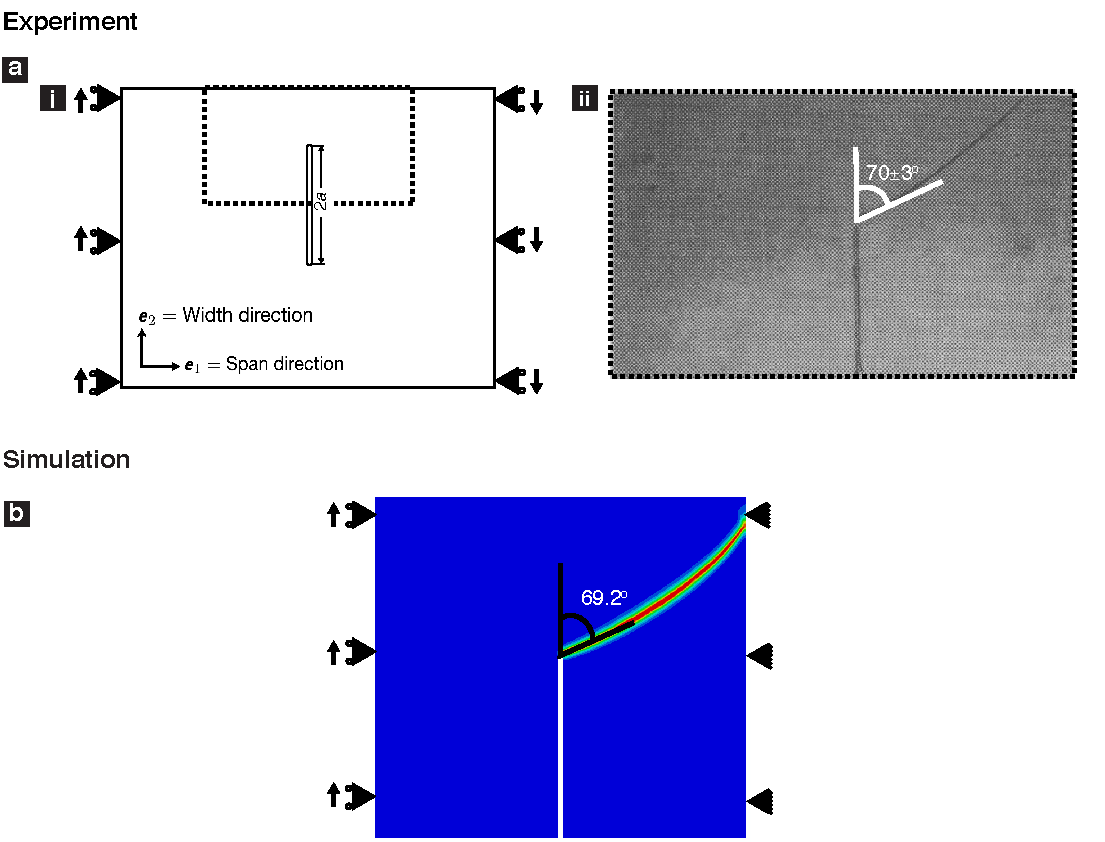
\includegraphics[width=\textwidth]{./Figures/Fig3_ver7.pdf}
	\caption{(a.i) An illustration of the geometry and the loading conditions in  Erdogan and Sih's experiments\cite{erdogan1963crack}. %hkdone
	(a.ii) A crack path from  Erdogan and Sih's experiments, as reported by Bittencourt \textit{et al.}~\cite{bittencourt1996quasi}. %hkdone
 (b) Our RVFT model of Erdogan and Sih's experiments and its predicted crack path. %hkdone
	% Simulations: E = 208*10^3 N/mm^2, \nu = 0.3, G_c = 1N/mm,  l = 0.012 mm, plane strain. In experiments:  0.12 in thick Plexi-glass, other dimensions not reported. Loading interpreted. 
	\label{fig:ErgodanSih}
	}
\end{figure}
%hkdone

We did consider including  the above discussion in the current manuscript in some form. However, we concluded that the current manuscript is perhaps not the appropriate forum for presenting our RVFT experimental validation results. Since presenting them in the supplementary information of the current manuscript would not do them justice considering their  significance. Presenting them in the main text would greatly change the scope of the manuscript, and make the manuscript  unfocused and lengthy. Therefore, with regard to our RVFT experimental validation results we decided to limit ourselves to the above discussion for the current manuscript. However, as we mentioned earlier, we plan on presenting them along with all the requisite details and background in our future publication that will exclusively focus on RVFT\footref{RVFTpaper}.
% hk done




\item \label{r2c12} {\bf ``Would for example, the fabrication and test of a simple synthetic analog, i.e. an artificial layered beam with controlled elastic properties for its bulk solid and its thin interlayer, be brought further evidence for the VFM accuracy and use in this work?''}

\begin{figure}[hb!]
	\centering
	\includegraphics[width=\textwidth]{./Figures/PMMA_Setup_7.pdf}
\caption{Specimens under preparation for experimental validation of RVFT. %hkdone
(a) \textit{Euplectella aspergillum}'s 2D synthetic analogues. %hkdone
Poly(methyl methacrylate)(PMMA) is laser-cut and glued back together to introduce weak interfaces perpendicular to the notch. %hkdone
(b)  \textit{Euplectella aspergillum}'s 3D synthetic analogue. %hkdone
A solid cylinder and a number of hollow cylinders of varying thicknesses and radii are 3D printed and assembled coaxially to resemble an \textit{Ea.} spicule.
(c) Fixture designed to conduct three-point bending test on the manufactured synthetic analogues.}
\label{fig:SyntheticAnalogues}
\end{figure}


Absolutely. %hk done, SK done
We too share the  Reviewer's interest in ascertaining the correctness/validity of  RVFT by carrying out controlled experiments and comparing their results with the predictions from RVFT models of those experiments. %hk done, SK done
The controlled experiments will involve  synthetic analogues of  \textit{Ea} spicules in which, e.g., the mechanical properties of the constituent materials and interfaces will be well known. %hk done, SK doneç
In fact, we have been trying to carry out such a comparison for the last two years. %hk done, SK done
For example, Figure~\ref{fig:SyntheticAnalogues} shows some of our  \textit{Ea} spicule synthetic analogues, which we manufactured using laser cutting and 3D printing. %hk done, SK done /$ $
Figure~\ref{fig:SyntheticAnalogues} (a) shows a two dimensional (2D) analogue that is very similar to the ``artificial layered beam with controlled elastic properties for its bulk solid and its thin interlayer'' that Reviewer \#2 talks about in their above comment (comment ~\ref{r2c12}). % hkdone
Figure~\ref{fig:SyntheticAnalogues} (b) shows a three dimensional (3D) analogue. %hkdone 
Figure~\ref{fig:SyntheticAnalogues} (c) shows the mechanical testing stage that we  designed and constructed for carrying out three-point bending fracture tests on our synthetic analogues. % hkdone
We discuss our 2D analogues further in the next paragraph. % hkdone

We created our 2D analogues by laser cutting PMMA sheets and gluing them together using solvent based adhesives. % hkdone
Thus, in our 2D  analogues the silica layers are represented by PMMA layers, and the protein interlayers (weak interfaces) are represented by the solvent based adhesive interlayers (PMMA-PMMA interfaces). % hkdone
Our aim is to measure the elastic properties and toughness of PMMA and the toughness of the PMMA-PMMA interfaces in our three-point bend tests, input those properties into RVFT models of our experiments, and compare the predictions from those models for, e.g., the load-displacement curves and cracks paths with those from our experiments. % hkdone
This is ongoing work and will take  one to two  years. % hkdone 

We believe that the conclusion of our experiments on synthetic analogues is not necessary for the publication of our current results. This is for the following two reasons:  %hkdone
(i) Firstly, as we discuss in our response to Reviewer \#2's comment~\ref{r2c1} we have already compared the predictions of RVFT with experimental observations  from three-point bending fracture tests conducted on SiC-graphite layered beams, which were reported by Clegg \textit{et al.}~\cite{clegg1990simple}. % hkdone 
(Those beams are very similar to the \say{artificial layered beam} that Reviewer \#2 mentions in their current comment (comment \ref{r2c12}).) % hkdone 
As we also discuss in our response to comment~\ref{r2c1}, we found from that comparison that RVFT is fully capable of making the type of qualitative predictions that we report in the manuscript. % hkdone 
(ii) Secondly, though very valuable in ascertaining the validity of RVFT, we believe that our ongoing study involving synthetic analogues is outside the scope of the current manuscript. %hkdone
Our primarily result---namely that  the toughness enhancement provided by the layered architecture is greatly suppressed in \textit{Ea.} spicules and hence architectural motifs in stiff biological materials may not be worthy of emulation by default, and they may not be benefiting a particular organism in the same way that they benefit a different organism--does not critically hinge on the insight provided by the RVFT simulations. %hkdone


 We thank  the Reviewer for pointing out a very interesting and important research direction. %hkdone



\item \label{r2c2} {\bf ``Furthermore, given the main gist of the discussion lies on the insights gained from the computational results, are there any limitations to point out on the validity of application of the VFM?''}

Indeed, there are several issues that limit RVFT's predictive capability. %hkdone
 In our opinion, the most important of such issues is RVFT's handling of compressive stresses. %hkdone
 
%  \begin{tcolorbox}[colback=blue!5,colframe=blue!75!black,title=To Do Max]
%  \begin{enumerate}
 
%  \item Need to make changes to SI to support our statement "Through change \ref{Mc1} we have added a new paragraph to Section S4.1 in which we describe this major limitation of RVFT (handling of compressive stresses)."
 
%  Perhaps a modification of the following  "We have carried out extensive simulations to experimentally validate our finite element implementation of the RVFT. The results from those simulations and similar results reported in literature (e.g. see ~\cite{mesgarnejad2015validation,miehe2010phase,wu2017phase}) make us feel confident that the  RVFT is a dependable tool for gaining qualitative insight into fracture mechanics related phenomena. %hk done
%  Needless to add, the RVFT does have several limitations with regard to its predictive capability, and requires further development before it is capable of making quantitative predictions. %hk done
%  For example, in RVFT, crack growth can occur in the presence of dominant local compressive stresses which is not physical. One of the most used strategies to circumvent this problem is Miehe et al.'s  tension-compression split\cite{miehe2010phase}. In this strategy the damage field $d$ affects only the positive part of the strain energy density, which is composed of only the positive eigenvalues of the strain tensor. However, we have found that this strategy predicts inaccurate crack paths in mixed-mode loading conditions and can lead to numerical artifacts in certain loading conditions. There have been several other strategies that have been proposed \cite{amor2009regularized,li2016gradient,strobl2016constitutive} to deal with compressive failure in RVFT, which remains an active area of research. We have done our utmost to ensure that the above discussed and related issues that are known to limit RVFT's predictive capability were absent or negligible in our  simulations."
% \item Need to mark $\boldsymbol{e}_1$ and $\boldsymbol{e}_2$ in Figure~\ref{fig:VRF-TCS}
% \item Check/fix red highlighted regions.
% \end{enumerate}
% \end{tcolorbox} %hkdone
 
A major issue in RVFT is that it does not distinguish between compressive and tensile stress states in dictating the nucleation and evolution of damage. This is because the evolution of $d$ is primarily governed by the strain energy density field, $\Psi_0$.  The only information about the deformation that appears in the governing equation for $d$ ( Eqn.~S25 in revised manuscript), is through $\Psi_0$. Thus, in the RVFT for the purposes of  dictating damage tensile and compressive stress states are indistinguishable when they correspond to the same strain energy density. Practically, what this means is that  a crack can form even under purely compressive loading, which of course is absurd. This feature essentially renders the RVFT unusable in many  important test cases. For example, consider the shear loading case shown in Figure~\ref{fig:VRF-TCS}.  A plate with an edge notch is subjected to in-plane shear loading. The boundary condition and loading are detailed in  Figure~\ref{fig:VRF-TCS}. As can be seen in subfigure (a), two crack branches emerge from the notch. The hoop stresses in the vicinity of the parent notch are compressive on the left side of the plate (see Figure~\ref{fig:VRF-TCS} (c)). Therefore, the left crack branch is clearly unphysical; it is an anomaly of the RVFT.
%hk done para


Crack growth under compressive loading poses a major problem for the application of RVFT.  However, a satisfactory solution to the problem of compressive failure is as yet unavailable.
%
For example, in order to overcome the compressive failure problem  Miehe et al.~\cite{miehe2010phase} proposed to split the strain energy density into a ``positive'', $\Psi_0^+$, and a ``negative'', $\Psi_0^-$, part.
%
The positive and negative parts are, respectively, constructed  using only the positive and negative eigenvalues of the strain tensor $\boldsymbol{\epsilon}$.
%
The strain energy term in the RVFT functional (Eq. S24 in the revised manuscript) is changed to $\int_{\mathcal{B}}g(d)\Psi_0^+ + \Psi_0^-d\mathcal{B}$ so  that now only $\Psi^+_0$ appears in the governing equation of $d$ instead of $\Psi_0$.
The intuitive thinking underlying   this strategy is that  the tensile and compressive stress states will predominantly only affect  $\Psi_0^+$ and $\Psi_0^-$, respectively.
%
Therefore, a compressive loading will not appreciably change $\Psi^+_0$ and cause $d$ to grow.
%
The splitting strategy does help to some extent.
%
For example, we repeated the shear loading test case using this strategy.
%
The results are shown in  Figure~\ref{fig:VRF-TCS} (b).
%
As can be see,  the anomalous left branch now no longer appears.
% hkdone para

However, the splitting approach is ad hoc, and lacks a rational mechanics justification.
%
Most importantly, we found that the splitting strategy, in some cases, introduces new anomalies of its own.
%
For example, consider the uniaxial tension test on a bar shown in Figure~\ref{fig:VRF-TCS} (d) that we performed using the splitting strategy.
%
As can be seen, damage has sporadically nucleated over the bar's length. This damage pattern in spurious;  an artifact of the splitting.
%
Thus, in summary, the strategy of splitting the strain energy density into a positive and negative part works in certain cases while in other cases it very manifestly introduces new anomalies.
%
A major point of concern therefore is the possibility that in some cases it  may introduce anomalies that are not as easy to identify as those shown in Figure~\ref{fig:VRF-TCS} (d) but which may lead to results that are significantly incorrect.
%hkdone para

As we stated in our response to Reviewer comment~\ref{r2c1}, we have done our utmost to ensure that the above discussed and related issues that are known to limit RVFT's predictive capability were absent or negligible in the  simulations that we report in the manuscript.
%hkdone para

In response to this comment we have made one change, which is listed as \ref{Mc1} in the \textit{LoC}.
%
Through change \ref{Mc1} we have added a new paragraph to Section S4.1 in which we describe this major limitation of RVFT (handling of compressive stresses).
%hkdone para




\begin{figure}[t!]
\begin{center}
  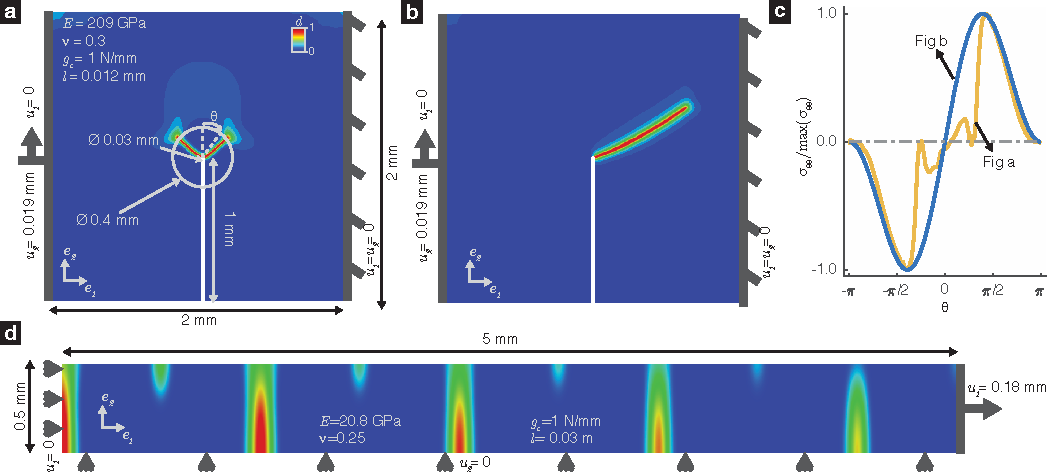
\includegraphics[width=\textwidth]{./Figures/TCsplit_V5.pdf}
    \caption{A limitation of RVFT: handling of compressive stresses. (a) shows the damage field on a  notched square plate that is subjected to in-plane shear loading. Specifically, the plate's right boundary is  encastered while a finite displacement is prescribed in  the $\boldsymbol{e}_2$ direction on the left boundary. The displacement in the $\boldsymbol{e}_1$ direction on the left boundary is set to zero. Material property and  geometry details are marked on the figure itself.  The damage field shows a single crack in the right half of the plate. (b) shows the results for the  same test case as  in (a) expect that here the calculation was performed using the splitting strategy.  The damage field now shows an additional, spurious branch on the left. (c) shows the hoop stresses, $\sigma_{\theta\theta}$, on a circle of radius 0.2 mm marked around the notch tip. The two different curves  correspond to simulations whose corresponding damage fields are  are shown in   (a) and (b). (d) shows the damage field for the case of a bar loaded in uniaxial tension. Symmetry boundary conditions are prescribed on the bottom and left boundaries of the bar. Displacements in the $\boldsymbol{e}_1$ and $\boldsymbol{e}_2$ directions on the right boundary  are prescribed to be $0.18$ and $0$ mm, respectively. The bar has no notches and in its initial state has no damage. We  solved this case using the splitting strategy, and  as can be seen damage has sporadically localized along the bar's  length.
		%hk done para
		}
      \label{fig:VRF-TCS}
\end{center}
\end{figure}








\item \label{r2c3} {\bf ``The term `specific fracture initiation toughness', an important concept the authors build upon in this work, initially appears in the fourth line of the text, but its formal definition comes to light only at pag 4. I suggest providing an informal definition of this term right when it appears for the first time. It doesn't need to be technical (at pag 4 there is already one), yet a few words to clarify the reader of this journal of broad audience what the authors refer to would certainly be an asset.''}

We agree with the Reviewer that the concept of fracture toughness should be defined earlier in the manuscript. In response to this comment we have made one change, which is listed as \ref{mc1} in the \textit{LoC}.
%
Through change \ref{mc1} we have added a new sentence in the first paragraph of the introduction that provides a basic definition of fracture initiation toughness.
%

\item \label{r2c4} {\bf ``Figure 3. i) Fig 3A. although quite clear, I would suggest adding the standard dash-dot line on the specimen geometry in A and B to indicate exactly where the circular cross-sections below are taken. ii) Fig 3C. References missing. I recommend including references in the caption for the data therein plotted. iii) Fig 3A seems uncalled in the text. The first instance I see is only for Fig 3B and 3C at line 58.''}

In response to this comment we have made one change, which is listed as \ref{mc2} in the \textit{LoC}.
%
Through change \ref{mc2} we have added the standard dash-dot line in subfigures 3A and 3B to indicate the location of the cross-sections. We have also added a reference to Figure 3A in the fourth paragraph of the introduction. Finally, we have identified the references from which the data in Figure 3C were obtained in the caption.

\item \label{r2c5} {\bf ``Figure 8. It seems the y axis is on log scale. If this is the case, I suggest indicating it on the axis and/or in the caption. In addition, also Fig 8A is not referenced in the text, only Fig 8b is at line 240.''}

In response to this comment we have made one change, which is listed as \ref{mc3} in the \textit{LoC}.
%
Through change \ref{mc3} we have modified the caption of Figure 8 to point out that the vertical axis has a logarithmic scale. We thank the Reviewer for this suggestion and think that pointing out that the vertical axis has a log scale reinforces the overall message of our work. We have also added a reference to Figure 8 (A) in the text of the revised manuscript  (in the second paragraph of Section 2.5 of the revised manuscript).%(in the fourth paragraph of the introduction). %Finally, we have identified the references from which the data in Figure 3C were obtained.

\item \label{r2c6} {\bf ``Figure 9. There seems to be an inconsistency with the choice of the view in Fig 9A and Fig 9B, the former displaying an axonometric view, whereas the latter is unclear (is it a front view?) because the cross-section on its right is a circle. How can this be? It should be an ellipse in an axonometric view, or I am missing something here. Another point on Fig 9F. Why at the notch location (bottom) a brown shaded zone appears? What is the physical meaning? Should the notch appear as open, as it is visible in the corresponding Fig. 9D?''}

The Reviewer is not missing anything here. As the Reviewer has identified, we made some mistakes in preparing Figure 9 (B) and 9 (F). In Figure 9 (B), the cross-section on the right should not be rendered as a circle. In Figure 9 (F) the notch should appear open, like in Figure 9 (D). We have rectified our mistakes in the revised manuscript, see change listed as \ref{mc4} in the \textit{LoC}. We thank the Reviewer for pointing out these mistakes. 

\item \label{r2c7} {\bf ``Statistics. This is a general comment that should be applied to relevant plots, table as well as text populated with data from this work or from the references. Statistical values are recommended for inclusion, where possible of course (if no data from the literature are available then the authors should nevertheless state this). The authors do a good job in providing mean values and standard deviations for the relevant mechanical property, e.g. line 173, but these values should be included also for the specimen geometry, so as to capture any discrepancy that might exist. For example, the start of the results section reports 25 Ea. and 12 Ta. Spicules were flexurally tested. But it seems no information (or I couldn't see) is given on the distribution of the geometric parameters that define these specimens. I would suggest including such information. I see much later in the text (pag 10) relevant values on the radius of curvature of the notch are given. Yet my comment here applies to the other main descriptors of the specimen geometry (cross-section radius, spicule length, layers thickness etc..). I would suggest including values of the specimen geometry up front in the results section, and use these raw values to build a short paragraph on the `specimen geometry characterization' showing any variations between data.''}

In response to this comment we have made three changes, which are listed as \ref{Mc2}--\ref{Mc4} in the \textit{LoC}.
%

Through change \ref{Mc2} we have included a new table (Table 1 in the revised version) that provides statistical data for our measurements of diameter ($D$), span ($L$), and notch length ($a$) for both the \textit{E. aspergillum} and \textit{T. aurantia} spicule specimens.
%
Through change \ref{Mc3} we have added the standard error of the notch root radius measurements to paragraph 4 of Section 2.3. This completes the inclusion of statistical data for specimen geometry.
%

Through change \ref{Mc4} we have modified Table 2 in the revised version (Table 1 in the original version). This table contains the crack growth resistance data (both $R(0)$ and $\left< R\right>$) used to compute the toughness metrics in Figure 8 for nacre, bone, antler, and conch shell. We have added statistical data such as mean, standard deviation, and sample number, when available. We have also clarified in the table footnotes when the number of specimens was not provided by a given reference or when the values in the table were estimated from graphs. We appreciate the Reviewer for pointing out this deficiency in our work.

\item \label{r2c8} {\bf ``A similar recommendation applies to the plot in S1 where the effect of moisture on the mechanical properties is given for 33 dry Ea and 11 wet Ea spicules. I suggest including in the caption the statistical output of the experiments to corroborate the claim that no difference in Young's modulus and strain failure emerges from the testing results. On this point, I also note here that the scatter of the green and the light blue bars shows some differences. Can the authors expand on the reasons please?''}

In response to this comment we have made one change, which is listed as \ref{mc5} in the \textit{LoC}.
%
Through change \ref{mc5} we have added the mean and standard error for the Young's modulus and bending failure strain of the wet and dry \textit{E. aspergillum} spicules to the caption of Figure S1. The statistical treatment of this data is handled in more detail in Section S2, where we use both bias-corrected accelerated confidence intervals and two-sided $t$-tests to corroborate our claim that there is no significant difference in effective Young's modulus or bending failure strain between the dry and wet spicules.

The difference in the scatter between the dry and wet spicules is most likely a consequence of the difference in sample number. That is, we only tested 11 spicules that were soaked in artificial seawater compared to the 33 dry spicules that were tested in \cite{monn2017enhanced}. The effect of hydration on the mechanical behavior of the \textit{E. aspergillum} spicules is certainly an important research topic, but a more in-depth treatment is beyond the scope of this work.

\item \label{r2c9} {\bf ``Line 76. The sentence `orthonormal set of Cartesian basis vectors $\{$e\string^1, e\string^2, e\string^3$\}$, shown in Figure 4 (A), (B), and (D), and their corresponding Cartesian coordinates $\{$x1, x2, x3$\}$'. Since fig 4 reports only the basis vectors without any display of the system $\{$x1, x2, x3$\}$, I would suggest to slightly amend the sentence as `orthonormal set of Cartesian basis vectors $\{$e\string^1, e\string^2, e\string^3$\}$ (Figure 4 (A), (B), and (D)), which correspond to the Cartesian coordinates $\{$x1, x2, x3$\}$'.''}

In response to this comment we have made one change, which is listed as \ref{mc6} in the \textit{LoC}.
%
Through change \ref{mc6} we modified the sentence in their comment above in the way suggested by the Reviewer so that it now reads ``The spicule specimen's undeformed configuration can be described using the orthonormal set of Cartesian basis vectors $\{\ex,\ey,\ez\}$ (Figure 4 (A), (B), and (D)), which correspond to the Cartesian coordinates $\{x_1,x_2,x_3\}$.''

\item \label{r2c10} {\bf ``Minor typos
In the main text: Line 276 layers, like that which appear >> like those? In the supplementary information: Line 14. That that >> avoid duplicate, Line 39. compare >> compared, Line 340. have been soaked >> were soaked, Reference 2 in the supplementary information lacks some data, such as the year.''}

In response to this comment we have made one change, which is listed as \ref{mc7} in the \textit{LoC}.
%
Through change \ref{mc7} we have corrected the typos identified by the Reviewer. We thank the Reviewer for identifying these small mistakes and allowing us to improve the quality of the manuscript.

\end{enumerate}

\clearpage
%%%%%%%%%%%%%%%%%%%%%%%%%%%%%%%%%%%%%%%%%%%%%%%%%%%%%%
\section*{Response to Reviewer \#3's comments}
\label{rev3}

\begin{enumerate}[label=\textit{3.\arabic*},wide, labelwidth=!, labelindent=0pt]
\item \label{r3c1} {\bf ``Now the authors gave an fairly extensive review on the studies reported until today by focusing on the toughness issues. However what I criticize is that the selection of the papers they cite is very ambiguous. The groups e.g. of Mayer, Fratzl, Weiner gave detailed report on this issue. Some pertinent report of these groups and also from others highlighted the importance of the proteins within the silica spicules and from the inter-layers.''}

Since this work focuses on the toughness properties of the \EA spicule, we focused our review on previous works that do the same. Many of these works have been published by Professor Mayer's group and are listed as references 5, 6, and 16 in the revised version of the manuscript. We do not agree that these references are ambiguous because, to our knowledge, they represent the main contributions to the study of the \EA spicules from the perspective of toughness enhancement via experimental measurements. The toughness properties of spicules with layered architecture produced by other species of the class Hexactinellida have been explored in references 19--22 and 54 in the revised version of the manuscript.

We agree with the Reviewer that Professor Fratzl's group and his collaborators (such as Professor Kolednik) have also made significant contributions to this subject. Their works primarily focus on modeling the effects of an elastically heterogeneous, layered architecture on initiation toughness. They propose a crack tip shielding effect that is caused by the interaction between a crack and an elastic heterogeneity. Through change \ref{Mc04} listed in the \textit{LoC} we have added an additional discussion of these works to Section 2.3 in the revised version of the manuscript. In this discussion, we describe the main premise of these models for toughness enhancement and point out how the analysis that we present in Section 2.5 constitutes a novel contribution by considering the cylindrical geometry of the \EA spicule's architecture. We have included references to the contributions of these groups, which are listed as references 8, 25, and 45--47 in the revised version of the manuscript.

To our knowledge Professor Weiner's group has not published any works on siliceous spicules (i.e. Demosponge or Hexactinellid spicules). Consequently, we have not included a review of their works in this manuscript. However, we do not deny the importance of the protein scaffold within the spicule's silica nor the composition of the interlayers. Our review of this topic focuses on the contributions of Dr. Weaver and Professor Aizenberg which are listed as references 17, 18, 43, and 54 in the revised version of the manuscript. These works describe the composition and nanoscale structure of the spicules' silica. We revisit the importance of the protein scaffold and composition of the silica itself in the final paragraph of Section 2.5. In this paragraph we point out that we chose the \TA spicules as a homogeneous control material based on the similarity of their composition and the composition of the \EA spicules. We admit that the best choice for this homogeneous control material would be the core of the \EA spicules themselves. However, we point out the difficulty of obtaining core samples large enough to test.

\item \label{r3c2} {\bf ``Also---importantly they mix spicules from demosponges with those from hexactinellids. This is not justified since the structure, composition of those spicules is different between these two taxa.''}

We agree that using spicules from the same taxonomic class would be the ideal choice. In fact, in Section 2.5 we state that ``The \EA spicules should instead be compared to a specimen composed of the same biogenic silica but which is monolithic. An ideal choice for this homogeneous control material would be a section of the solid silica core of the \EA spicules. However, so far we have not successfully obtained a large enough section of the \EA spicule core to perform fracture tests. Therefore, we chose the \TA spicules as what we believe to be the next best alternative.''

We used the \TA spicules specifically as a material for comparison since they have been shown to have a similar volume-averaged bonding structure to the \EA spicules \cite{weaver2010unifying}. Specifically, $^\text{29}$Si MAS NMR spectra of the \EA and \TA spicules indicate no distinguishable differences in the condensation of their silica. While this does not rule out differences in the proteinaceous scaffold, it does give a clear indication that the \TA spicules are a close approximation in terms of silica composition. We have also measured the Young's moduli of both the \EA and \TA spicules via three-point bending tests and found no significant difference between the two. This indicates that the elastic moduli of the silica from the \EA and \TA spicules are similar.

We agree with the Reviewer that differences in spiculogenesis between hexactinellids and demosponges will cause structural differences between the \EA and \TA spicules. We believe that this work constitutes a substantial improvement over past works focusing on toughness because it is the first to compare the \EA spicules to spicules from a related sponge instead of to synthetic glass. We hope that this work will motivate the importance of continuing to seek better control materials for comparison, such as sections of the \EA spicule core.

\item \label{r3c3} {\bf ``I the authors would stick to one taxon---then they surely will come to another conclusion. Then the issue, basically two issues, become more clear.''}

Regarding the conclusions of our work, we can assess the \EA spicule's toughness enhancement by analyzing the data we present for the \EA spicules alone. Specifically, by taking the ratio of $\left< R\right>$ to $R(0)$ for the \EA spicules we can quantify the rise in their $R$ curve during the propagation of a crack. This gives a rough sense of the effect of the \EA spicule's architecture on its toughness during crack propagation through what are considered ``extrinsic'' toughening mechanisms (see \cite{evans1990perspective}). For the \EA spicules, this ratio is approximately 22. We can compute this ratio for other biological materials using values found in Table 2. The values of $\left< R\right>/R(0)$ for nacre, bone, antler, and conch are 3.5, 56.3, 140.0 and 1040.0, respectively. Thus, even without comparing to the \TA spicules we can see that the increase in $R$ provided by the \EA spicule's architecture is significantly smaller than most of these other biological materials.

We do not know what two issues the reviewer is referring to in their comment.

\item \label{r3c4} {\bf ``I do not see any new ideas on the toughness of the layered mineralic biomaterials.''}

The main conclusion and significance of our work is as follows. In the biomimetics and bioinspired engineering communities, the \EA spicule's layered architecture is being linked to potential toughness enhancement by default without direct experimental evidence to support that link~\cite{mayer2011new, mayer2005rigid, kolednik2011bioinspired, walter2007mechanisms}. Our primary conclusion is that due to its cylindrical nature, the \EA spicule's layered architecture provides relatively little toughness enhancement compared to other biological materials, such as nacre and conch shell.

Specifically, we found that in comparison to nacre, the initiation toughness and average crack growth resistance enhancements provided by the \EA spicule's layered architecture are smaller by a factor of 100 and 60, respectively. Thus, despite the layered architecture in \textit{Ea.} spicules appearing very similar to those in nacre and conch shell---all three consist of micrometer thick ceramic/mineral layers glued together by nanometer-thin, soft, proteinaceous materials---and the \textit{Ea.} spicules appearing to serve similar functions as nacre and conch shell---all three are stiff, marine, biological materials that serve structural functions in the organisms that create them---the layered architecture provides far less toughness enhancement for \textit{Ea. spicules} than it does for nacre or conch shell. The stark contrast between the toughness enhancements observed in the \EA spicules and in these other materials demonstrates that the details of a material's layered architecture (e.g., flat vs cylindrical layers) can have extreme consequences on the toughening mechanisms that it enables and the resulting toughness enhancement it provides.

This is a very important finding, since it means that an architectural motif may not be benefiting a particular organism to the same degree that it does other organisms. In fact, the same architectural motif may be tied to different properties in different organisms, or not be tied to any property at all and just be a side effect of growth processes. The overarching implication is that the observation of an architectural motif's benefit in one biological material does not justify its use as a general template for reproducing that biological material's remarkable property enhancement in synthetic materials.

\item \label{r3c5} {\bf ``The authors gave a very attractive title for their manuscript---but they failed to give the readers an answer to: ``\ldots or a Siren Song.'' Just to mention that more conclusive results have to be worked out in the future is not sufficient.''}
\end{enumerate}

The title of the manuscript is meant to reflect the contrast between our findings and the widespread belief that biological materials with layered architectures have extraordinary fracture toughness. While we do state that ``the contrast between our findings and previous speculations that the \EA spicule's layers enhance their toughness shows that the understanding of the relationship between layered architectures and toughness enhancement is not yet complete'', we provide much more concrete conclusions as well. We enumerate some of the most important conclusions below.
%
\begin{enumerate}
    \item The \EA spicule's cylindrically layered architecture provides up to 10 fold increase in fracture initiation toughness. While this is certainly significant, it pales in comparison to the 200 fold increase observed in nacre (see Figure 8 (a)).
    \item Perhaps more importantly, the increase in average crack growth resistance provided by the \EA spicule's architecture is 60 times smaller than that provided by nacre's layered architecture.
    % \item Using a regularized variational fracture method, we found that interfacial fracture is the dominant toughening mechanisms in the cylindrical layered architecture, but that its effect is small compared to the arrest and re-nucleation mechanism that occurs in a planar layered architecture.
\end{enumerate}
%
We do not believe that the answer to the question posed in our title (i.e., are architectures in stiff biological materials a template for toughness or a siren song?) has a single, definitive answer. In conch shell, the crossed lamellar architecture clearly provides extraordinary enhancements to average crack growth resistance. In nacre, the brick and mortar architecture does the same for fracture initiation toughness. In the \EA spicules, the cylindrically layered architecture only provides modest enhancements to both. While at first glance, all of these materials have similar architectures, however, the seemingly small architectural differences lead to quite different fracture toughness properties. Sometimes these properties are extraordinary, sometimes they are not. Addressing that subtlety is the main point of this work.

\clearpage
%%%%%%%%%%%%%%%%%%%%%%%%%%%%%%%%%%%%%%%%%%%%%%%%%%%%%%
\bibliographystyle{apalike}
\bibliography{revbib}
\end{document}

% Hence, our conclusion is not what Reviewer \#1 believes it is.  

% As a consequence of the above misunderstanding, Reviewer \#1 appears to believe that our findings are at odds with the works of Kolednik \textit{et al.},  Fratzl \textit{et al.}, and Sistaninia \textit{et al.}~\cite{fratzl2007hindered, kolednik2011bioinspired, kolednik2014improvements, sistaninia2018design}. Our conclusion is not at odds with the results of the works of Fratzl \textit{et al.} In fact our work is in perfect agreement with the works of Fratzl \textit{et al.} and provides further support to their works. As per the works of Fratzl \textit{et al.}, the lamellar structure is supposed to enhance initiation toughness. This is exactly what our experiments found. We reported this enhancement in Figure 8 (A). Specifically, we found that the \EA spicule's cylindrically layered architecture on average provided a 7\% enhancement to the spicule's initiation toughness.   

% (as per the results of x), i.e., and it is not valid to combine data corresponding to different $\alpha$ values to perform the statistical test.
%  From the load-displacement response of the SiC-Graphite composite shown in Figure~\ref{Fig1}(b), it was found that the toughness of the composite was substantially higher than monolithic SiC. Using our RVFT, we have performed three point bending simulations on SiC-Graphite-type architectures. In our simulations, we assigned SiC layers a toughness of $G_b = 0.5$ N/mm and the Graphite interlayers a toughness of $G_I = 0.05$ N/mm (see Figure~\ref{Fig1}(c)). The simulations showed that toughness enhancement mechanism is crack deflection and arrest at the Graphite interfaces followed by crack reinitiation at the subsequent SiC layers. The crack path for the case of three interlayers is shown in Figure~\ref{Fig1}(c), where the red region (i.e., the damage field $d \approx 1$) indicates the cracked region. We performed these simulations for different number of interlayers and the load-displacement response corresponding to 0,1,2,3 and 4 interlayers is shown in Figure~\ref{Fig1}(d). On comparing the load-displacement from the experiment in subfigure(b) and from RVFT in subfigure(d), we can see that RVFT predicts the zigzag load-displacement response seen in the experiments. Thus, we can conclude that RVFT can qualitatively predict crack patterns toughness enhancement mechanisms in 2D layered architectures.

% {}
% For the reasons we gave in our response to Reviewer \#2' comment~\ref{r2c1} we believe that 

% We believe that further investigation of the cylindrical layered architecture through the use of synthetic analogs would give deeper insights into the toughening mechanisms acting within the spicules. Furthermore by varying the curvature of the layers one may be able to better understand the transition of toughening mechanisms from those operating in planar layered architectures to those operating in cylindrical layered architectures.


% as formulated in Section S4 is that the material(s) in the model are ideally brittle (i.e., they have a small fracture process zone). The are two major limitations/issues that we have identified for the RVFT framework for brittle materials, (i) crack growth due to local compressive stresses and, (ii) computational expense.